\documentclass[titlepage, a4paper, openbib, 10pt]{article}

%#####################################
%Usepackages en installingen
\usepackage[top=1in, bottom=1in, left=1in, right=1in]{geometry}
\usepackage[pdftex]{graphicx}
\usepackage{fancyhdr}
\usepackage{sectionbox}
\usepackage[dutch]{babel}
\usepackage{chngcntr}
\usepackage{cite}
\usepackage{url}
\usepackage{makeidx}
\usepackage{paralist}
\usepackage{enumitem}
\usepackage{tocloft}
\usepackage{listliketab}	
\usepackage[table]{xcolor}
\usepackage{tabularx}
\usepackage{epsfig}
\usepackage{pdflscape}
\usepackage{pdfpages}
\usepackage{float}
\usepackage{amsmath}
\usepackage{comment}
\usepackage{multirow} 
\usepackage{rotating}
\usepackage[utf8]{inputenc}
\usepackage{color}
\newcommand{\red}[1]{
\textcolor{red}{#1}
}
\usepackage{verbatim}
\usepackage{listings}
\lstset{language=C,
basicstyle=\ttfamily\footnotesize,
frame=shadowbox,
mathescape=true,
showstringspaces=false,
showspaces=false,
breaklines=true}


%\usepackage{showframe} %tmp
%#####################################
%Nieuwe commando's
\newcommand{\HRule}{\rule{\linewidth}{1pt}}
\newcommand{\organisatie}{\uppercase{Hogeschool Rotterdam / CMI}}
\newcommand{\modulenaam}{Algorithms}
\newcommand{\modulecode}{\uppercase{INFDEV026A}}
\newcommand{\stdPunten}{4 ects}
\renewcommand{\author}{G. Costantini}

\definecolor{lichtGrijs}{RGB}{169,169,169}



%#####################################
%Index en styling
\setlength{\cftbeforesecskip}{10pt}
\setlength\parindent{0pt}
\makeindex
\graphicspath{{img}}
\counterwithin{figure}{subsection}
\pagestyle{fancy}
\setcounter{secnumdepth}{5}
\setcounter{tocdepth}{5}

%#####################################
%     Alles voor header/footer
\fancyhf[HL]{\nouppercase{\textit{\leftmark}}}
\setlength{\headheight}{36pt}
\lhead{\uppercase{\footnotesize Course description}}
\chead{\footnotesize \organisatie}
\rhead{
\includegraphics[width=0.09\textwidth]{img/logo}}

\lfoot{\scriptsize \modulenaam}
\cfoot{\scriptsize \today}
\rfoot{\small \thepage}

\renewcommand{\headrulewidth}{0.4pt}
\renewcommand{\footrulewidth}{0.4pt}
%#####################################

\begin{document}

%#####################################
%Titlepage
\begin{titlepage}
\thispagestyle{fancy}
\ 
\vspace{5cm}

\begin{center}

	
	\Large \textbf \organisatie
	
	\vspace{1.5cm}
	
	\HRule \\[0.4cm]
	
	\Huge \textbf \modulenaam
	
	\vspace{1.7cm}
	
	\Large \textbf  \modulecode
	
	\vspace{0.4cm}
	
	\HRule \\[1.5cm]
\end{center}
\vfill

% Author and supervisor
\begin{tabular}{l l}
	Number of study points:  & \stdPunten\\
	Course owners: & \author\\
\end{tabular}

\end{titlepage}

%####### Contentpagina ########
%\renewcommand{\baselinestretch}{1.5}\normalsize
%\tableofcontents
%\newpage
%\listoffigures
%\newpage
%\listoftables
%\newpage

%########### Inhoud ###########

\shadowsectionbox
\section*{Module description}
\begin{tabularx}{\textwidth}{|>{\columncolor{lichtGrijs}} p{.26\textwidth}|X|}
	\hline
	\textbf{Module name:} & \modulenaam\\
	\hline
	\textbf{Module code: }& \modulecode\\
	\hline
	\textbf{Study points \newline and hours of effort for full-time students:} & This module gives \stdPunten, in correspondance with 112 hours:
	\begin{itemize}
		\item 2 x 8 hours frontal lecture
		\item 3 x 8 hours self-study for the theory
		\item the rest is self-study for the practicum
	\end{itemize} \\
	\hline
	\textbf{Examination:} & Written examination and practical assignment (with oral check) \\
	\hline
	\textbf{Course structure:} & Lectures \\
	\hline
	\textbf{Prerequisite knowledge:} & Object oriented programming \\
	\hline
	\textbf{Learning tools:} & \begin{itemize}
			\item Book: \textit{Algorithms} (4rd edition); authors R. Sedgewick, K. Wayne
			\item Lesson slides (pdf): found on N@tschool
			\item Assignments, to be done at home (pdf): found on N@tschool
		\end{itemize} \\
	\hline
	\textbf{Connected to \newline competences:} & \begin{itemize}
			\item Realisation
			\item Analysis
		\end{itemize} \\
	\hline
	\textbf{Learning objectives:} &
		At the end of the course, the student can:
			\begin{itemize}
				\item do performance analysis [\texttt{PERF}]
				\item implement and analyse 
					\begin{itemize}
						\item basic data structures [\texttt{DS}\textsuperscript{I}, \texttt{DS}\textsuperscript{A}]
						\item sorting algorithms [\texttt{SORT}\textsuperscript{I}, \texttt{SORT}\textsuperscript{A}]
						\item recursive data structures [\texttt{REC}\textsuperscript{I}, \texttt{REC}\textsuperscript{A}]
						\item algorithms on graphs [\texttt{GRAPH}\textsuperscript{I}, \texttt{GRAPH}\textsuperscript{A}]
					\end{itemize}
			\end{itemize} \\
	\hline

%\end{tabularx}
%\begin{tabularx}{\textwidth}{|>{\columncolor{lichtGrijs}} p{.26\textwidth}|X|}
%	\hline
	\textbf{Course owners:} & \author\\
	\hline
	\textbf{Date:} & \today \\
	\hline
\end{tabularx}
\newpage


\section{General description}
	Designing and manipulating efficient data structures is at the foundation of computer programming. 
	These data structures solve complex problems through well-known, highly difficult techniques that would simply take too long to rediscover from scratch. When faced with certain classes of issues, lack of knowledge of algorithms and data structures might significantly impact a programmer's ability to tackle a given problem. \\	
	In this course we are going to explain some of the most popular data structures used in a variety of scenario's encountered in practice when dealing with structuring and traversal of data. 
	We will also cover the principal pathfinding algorithms, which are extensively used for example in GPS devices, routers, etc.  \\

	\subsection{Relationship with other teaching units}
		This course builds upon the development courses of the first year.	\\		

		Advanced data structures presented in this course are used in the optimization of RDBMS's and are informally presented during INFDEV03-5. They play a role in data analysis, simulations, optimization of code, and many others. \\
		
		Knowledge acquired through the algorithms course is also useful for some of the projects. A word of warning though: projects and development courses are largely independent, so some things that a student learns during the development courses are not used in the projects, some things that a student learns during the development courses are indeed used in the projects, but some things done in the projects are learned within the context of the project and not within the development courses.


\section{Course program}
	
	In the following table you can see the program of the course, divided per lesson. Each lesson is also associated to the corresponding book paragraphs. The last lesson of the course is reserved for a summary in preparation for the exam. \\
	
	\begin{tabular}{ | p{1.2cm} | p{10cm} | p{3.7cm} | }
		\hline
	  	\textbf{Lesson} & \textbf{Topic} & \textbf{Book paragraphs} \\
	  	\hline
  		1 & Arrays; Complexity of algorithms (empirical analysis, O notation) & 1.4 \\
  		\hline
  		2 & Sorting algorithms (insertion sort, mergesort) & 2.1, 2.2 \\
  		\hline
  		3 & List, Queue, Stack, Hash table & 1.3, 3.4 \\
  		\hline
  		4 & Trees (BST, k-d trees, 2-3 trees) & 3.2, 3.3 \\
  		\hline
  		5 & Graphs (undirected; directed; Dijkstra shortest path) & 4.1, 4.2, 4.4 \\
  		\hline
  		6 & Dynamic programming; Floyd-Warshall & Not covered by the book, see slides or Cormen\\
  		\hline
  		7 & Practicum / reserve lesson & \\
  		\hline
  		8 & Course recap & \\
  		\hline
	\end{tabular}
\begin{comment}
  		4 & Binary search trees & 3.2 \\
  		\hline
  		5 & Balanced search trees: 2-3 search trees & 3.3 \\
  		\hline
  		6 & Graphs (undirected; directed; Dijkstra shortest path) & 4.1, 4.2, 4.4 \\
  		\hline
  		7 & Dynamic programming; Floyd-Warshall & Not covered by the book, see slides or Cormen\\
  		\hline
  		8 & Course recap & \\
  		\hline
\end{comment}


\section{Assessment}
	The course is tested with two exams: a practical examination and a theoretical examination. The final grade is determined by the practical examination. However, to receive the grade in the practical examination you \textbf{must} have a sufficient (i.e. $\geq$ 5.5) grade in the theoretical examination.

	\subsection{Theoretical examination}
		The theoretical examination consists of a \textbf{written exam} which covers the topics seen in class. The questions will be both theoretical and about code analysis, such as understanding what a code snippet does, determining its complexity, or finding mistakes in it.
		The exam lasts two lesson hours (100 minutes). No help is allowed during the exam.\\
		A template of the exam can be found in Attachment 1.

	\subsection{Practical examination}
	The practical examination is a \textbf{programming assignment}, accompanied by a brief \textbf{oral check} (to verify the authorship of code). In the practical assignment, some of the data structures and algorithms seen in class will have to be implemented and applied to a specific case study.\\ 
	A detailed description of the practical assignment can be found in Attachment 2.
%	Important notes:
%	\begin{itemize}
%	\item The assignment must be done individually.
%	\item You must upload your project on Github and (only at the end) on N@tschool. The teachers must be added to the Github repository. 
%	\item Each exercise of the practical assignment is associated to a specific deadline. The intermediate deadlines will be checked through the commits in Github.
%	\item There will be oral checks to verify the authorship of code.
%	\item The framework for the assignment comes only for .NET languages: allowed languages are C\# and F\#.
%	\end{itemize}
	
	\subsection{Retake (herkansing)}
	If one part of the assessment is not sufficient (theoretical and/or practical examination), then you can repeat that part in the following block:
	\begin{itemize}
	\item In week 10 of the following block you can repeat the written exam.
	\item The deadline for the delivery of the practical examination is at the end of week 9 of the following block.
	\end{itemize}
	


%\bibliographystyle{plain}
%\bibliography{references}
%\newpage
\section*{Attachment 1: Written exam template}
The general shape of a written exam for this course is made up of a series of highly structured open questions.

\paragraph*{Question I: complexity} \ \\

\textbf{General shape of the question:} \textit{Given the following code, what is its (tightest) complexity class using the big-Oh notation?} \ 

\textbf{Grading:} \textit{2 points for correct answer, 0 otherwise.} \ 

\textbf{Associated learning goals:} \texttt{PERF}.

\ \\ 
\paragraph*{Question II: basic data structures (list, queue, stack, hash tables)} \ \\

\textbf{General shape of the question:} \textit{Complete the code below so that it produces the desired result on the specified basic data structure.} \ 

\textbf{Grading:} \textit{2 points for correct answer, 1 point for minor mistakes, 0 otherwise.} \ 

\textbf{Associated learning goals:} \texttt{DS}\textsuperscript{A}.

\ \\ 
\paragraph*{Question III: sorting} \ \\

\textbf{General shape of the question:} \textit{What is the output of the following algorithm if input is ... ? What is the (tightest) complexity class of the algorithm (using the big-Oh notation)?} \ 

\textbf{Grading:} \textit{2 points for correct complexity and output, 1 point for either correct complexity or output, 0 otherwise.} \ 

\textbf{Associated learning goals:} \texttt{SORT}\textsuperscript{A}.

\ \\ 
\paragraph*{Question IV: trees} \ \\

\textbf{General shape of the question:} \textit{Complete the code below so that it produces the desired result (for example, insertion, lookup, traversal, ...) on a tree.} \ 

\textbf{Grading:} \textit{2 points for correct answer, 1 point for minor mistakes, 0 otherwise.} \ 

\textbf{Associated learning goals:} \texttt{REC}\textsuperscript{A}.

\ \\ 
\paragraph*{Question V: graphs} \ \\

\textbf{General shape of the question:} \textit{What does the following algorithm produce? What is the (tightest) complexity class of the algorithm (using the big-Oh notation)?} \ 

\textbf{Grading:} \textit{2 points for correct complexity and output, 1 point for either correct complexity or output, 0 otherwise.} \ 

\textbf{Associated learning goals:} \texttt{GRAPH}\textsuperscript{A}.

\ \\ 



%%%%%%%%%%%%%%%%%%%%%%%%%%%%%%%%%%%%%%%%%

\begin{comment}
	\begin{tabular}{|p{3cm}|p{3.5cm}|p{6cm}|}
		\hline
		\textbf{Learning goal} & \textbf{Dublin descriptors} & \textbf{Tested through} \\
		\hline
		\texttt{KNOW} & 1 & Theoretical examination \\
		\hline
		\texttt{IMPL} & 2 & Practical examination \\
		\hline
		\texttt{AN} & 3 & Theoretical examination \\
		\hline
		\texttt{APP} & 2, 3 & Theoretical and practical examination \\
		\hline
	\end{tabular}
	
	\vspace{1cm}

	Dublin-descriptors:
	\begin{enumerate}
		\item Knowledge and understanding
		\item Applying knowledge and understanding
		\item Making judgements
		\item Communication
		\item Learning skills
	\end{enumerate}
\end{comment}
\newpage
%/\include{tex/Practicums}
%/\newpage
%/\section*{Exam structure}
What follows is the general structure of a DEV5 exam.
\\ 
\\
\textbf{Associated learning goals:} \texttt{ORM}, \texttt{RDBMS}.
\textbf{Points:} \textit{25\%.}
\paragraph{Question I: SQL queries} \ \\

\textit{Given a database definition writes the SQL code for the requested queries} 

\ \\


\textbf{Answer:} \textit{}

\begin{lstlisting}
\end{lstlisting}


\ \\ 
\textbf{Associated learning goals:} \texttt{OPT}, \texttt{RDBMS}.
\textbf{Points:} \textit{25\%.}
\paragraph{Question II: Query optimization in SQL} \ \\ 

\textit{Given the following queries identify at least N-columns to be indexed with suitable index}

\begin{lstlisting}
\end{lstlisting}

\ \\ 

\textbf{Associated learning goals:} \texttt{TRANS-CONS}, \texttt{RDBMS}.
\textbf{Points:} \textit{25\%.}
\paragraph{Question III: Transaction management and concurrency}

\ \\ 

\textit{Given the following N-queries, which are run in parallel, show plausible solutions }
\begin{lstlisting}
\end{lstlisting}

\ \\ 

\textbf{Answer:} \textit{...}


\ \\ 
\textbf{Associated learning goals:} \texttt{NON-REL}.
\textbf{Points:} \textit{25\%.}
\paragraph{Question IV: Crash recovery}

\ \\ 

\textit{Given the following log file explain the behaviour of the crash recovery and the UNDO/DO phases}

\begin{lstlisting}
\end{lstlisting}

\ \\ 
\textbf{Associated learning goals:} \texttt{NON-REL}.
\textbf{Points:} \textit{25\%.}
\paragraph{Question V: NoSQL databases en Graph Theory}

\ \\ 

\textit{Transoform this relational data model into a graph model OR given this un-/directed graph identify the adjancy list or matrix of it}

\begin{lstlisting}
\end{lstlisting}

\ \\ 

\textbf{Concrete example of answer:} \textit{}

\ \\ 
\textbf{Grading:} \textit{All values are correct: full-points. At least half the values are correct: half points. Zero points otherwise.}

\ \\ 

%/\newpage
%\section*{Exam sample}
What follows is a concrete example of the exam.


\paragraph{Question I: formal rules} \ \\

\textit{You start at point (0,0). Take a step in the direction (10,0) until you are above point (45,0). Then take five steps in the direction (0,2). Where do you end up?}

\ \\ 

\textbf{Answer:} \textit{The trajectory is:}

\begin{lstlisting}

P1 = (50,0)
 +----- P2 = (50,10)
 |
 |
 |
 |
P0 = (0,0)
\end{lstlisting}

\ \\ 

\textbf{Points:} \textit{25\%.}

\ \\ 
\ \\ 

\paragraph{Question II: program state} \ \\ 

\textit{Fill-in the program state with the values that the variables assume while running the sample below.}

\begin{lstlisting}
y = 1
for i in range(0, 5):
    y = y * 2
\end{lstlisting}

\ \\ 

\textbf{Answer:} \textit{The variable allocations are:}

\begin{tabular}{| c | c | c | c | c | c | c | c |}
\hline
\textbf{y} & 1 & 1 & 2 & 4 & 8 & 16 & 32 \\
\hline
\textbf{i} & n.a. & 0 & 1 & 2 & 3 & 4 & 4 \\
\hline
\end{tabular}

\ \\
s
\textbf{Points:} \textit{25\%.}

\ \\ 

\textbf{Grading:} \textit{Full points if all values are correctly listed in the right order. Half points if at least half of values are listed in the right order. Zero points otherwise.}

\ \\ 

\textbf{Associated learning goals:} \texttt{CMC}.

\ \\ 

\paragraph{Question III: variables, expressions, and data types}

\ \\ 

\textit{What is the value and the type of all variables after execution of the following code?}
\begin{lstlisting}
v = 0
i = "Hello + world"
j = "Hello" + "world"
k = 10 / 3
\end{lstlisting}

\ \\ 

\textbf{Answer:} \textit{The value and type of all variables after execution is:}

\begin{tabular}{| l | c | c | }
\hline
\textbf{Variable} & \textbf{Value} & \textbf{Type} \\
\hline
v & 0 & int \\
\hline
i & 'Hello + world' & str \\
\hline
j & 'Helloworld' & str \\
\hline
k & 3 & int \\
\hline
l & 3.3333$\dots$ & float \\
\hline
\end{tabular}

\ \\ 

\textbf{Points:} \textit{25\%.}

\ \\ 

\textbf{Grading:} \textit{All values and types are correct: full-points. At least half the values and at least half the types are correct: half points. Zero points otherwise.}

\ \\ 

\textbf{Associated learning goals:} \texttt{VAR}, \texttt{EXPR}.

\ \\ 

\paragraph{Question IV: control flow}

\ \\ 

\textbf{General shape of the question:} \textit{What is the value of all variables after execution of the following code?}

\ \\ 

\textbf{Concrete example of question:} \textit{What is the value of all variables after execution of the following code?}

\begin{lstlisting}
v = 0
for i in range(1,15):
  if (i % 2 == 0) & (i % 3 == 0):
    v = v + i
\end{lstlisting}

\ \\ 

\textbf{Concrete example of answer:} \textit{The value of all variables after execution is:}

\begin{tabular}{| l | c |}
\hline
\textbf{Variable} & \textbf{Value} \\
\hline
\texttt{i} & \texttt{14} \\
\hline
\texttt{v} & \texttt{18} \\
\hline
\end{tabular}

\ \\ 

\textbf{Points:} \textit{25\%.}

\ \\ 

\textbf{Grading:} \textit{All values are correct: full-points. At least half the values are correct: half points. Zero points otherwise.}

\ \\ 

\textbf{Associated learning goals:} \texttt{COND}, \texttt{LOOP}.

\ \\ 

%##############################

%\newpage
\section*{Attachment 2: Practical examination}

\subsection*{General (important) information}
\begin{itemize}
\item The assignment is individual.
\item The assignment must be implemented using C\# or F\#.
%\item Not delivering the assignment in time implies taking the exam at the retake.
\item The only library tools you are allowed to use are: arrays, lists, and math functions. Other data structures or functions on data structures covered by the course must be implemented \textbf{by hand}.
\item There will be a brief \textbf{oral check} on the content of the assignment.
\item The grade is given by the sum of the grades obtained in each exercise, plus 1.
\item \textbf{Deadlines and delivery}
\begin{itemize}
\item Each exercise has a (strongly) suggested deadline.
\item You must use \textit{Github} and do frequent commits. The amount/time of the Github commits \textit{could} be checked by the teachers and considered as grading evidence, for example in case of a borderline grade.
\item By the \textit{end of week 9}, you must upload your project on \textit{N@tschool} (through the ``inleveropdracht").
\end{itemize}
\end{itemize}

\subsection*{Introduction to the framework}
The exercises will be based on the simulation of a city, containing houses and special buildings (represented through ancient civilization temples), all connected by streets. The student must implement algorithms to answer some queries on the simulated city.
To set up the framework, follow these instructions:

\begin{itemize}
\item Download and install Visual Studio 2015 Community (\url{https://www.visualstudio.com/en-us/downloads/download-visual-studio-vs.aspx}); choose ``F\# language" during \textit{custom setup}; 
\item Download the project framework from N@tschool (or Github) and open the .sln file; if it is not already set, right click on \texttt{EntryPoint} project (in the solution explorer) and select ``Set as startup project";
\item The functions you have to program are contained in the file \texttt{Program.cs}; for now there are stub versions of the function implementations that you have to replace with yours;
\item Compile the project in debug mode and run it with Ctrl+F5;
\item A window opens asking you which assignment you want to execute: choose a number between 1 and 4 \footnote{In the application, assignment 3 corresponds to exercise 3.1; assignment 4 corresponds to exercise 3.2.} (or q if you want to close it) and press Ok;
\item The simulation will start. You can move the visual with WASD and zoom with Z (zoom in) and X (zoom out).
\item Exit with ESC. 
\end{itemize}

\newpage
\subsection*{Exercise 1 - Sorting}

\textbf{Suggested deadline}: End week 4. \\
\textbf{Points}: 3.

\subsubsection*{Goal}
Sort all special buildings by Euclidean distance from a specified house. The Euclidean distance formula is:
\begin{align*}
d(house,building) = \sqrt{(x_{house} - x_{building})^{2} + (y_{house} - y_{building})^{2} } 
\end{align*}
This means that the connection through roads is not relevant in this exercise (everyone has his private helicopter to move around the city).

\subsubsection*{Function signature} 
\begin{lstlisting}
private static IEnumerable<Vector2> SortSpecialBuildingsByDistance(Vector2 house, IEnumerable<Vector2> specialBuildings)
\end{lstlisting}

This function takes as input a house position (\texttt{Vector2 house}) and a list of building positions (\\ \texttt{IEnumerable<Vector2> specialBuildings}) and returns a sorted list of building positions according to their distance from the house position (\texttt{IEnumerable<Vector2>}). Use the \textbf{merge sort} as sorting algorithm. Any implementation not using this technique will not be accepted and evaluated.\\

\subsubsection*{Result}
As you can see from Figure \ref{img:Ex1}, the selected house is highlighted and there is a number above each special building indicating its position in the sorted list of buildings. 

\begin{figure}[!h]
\centering
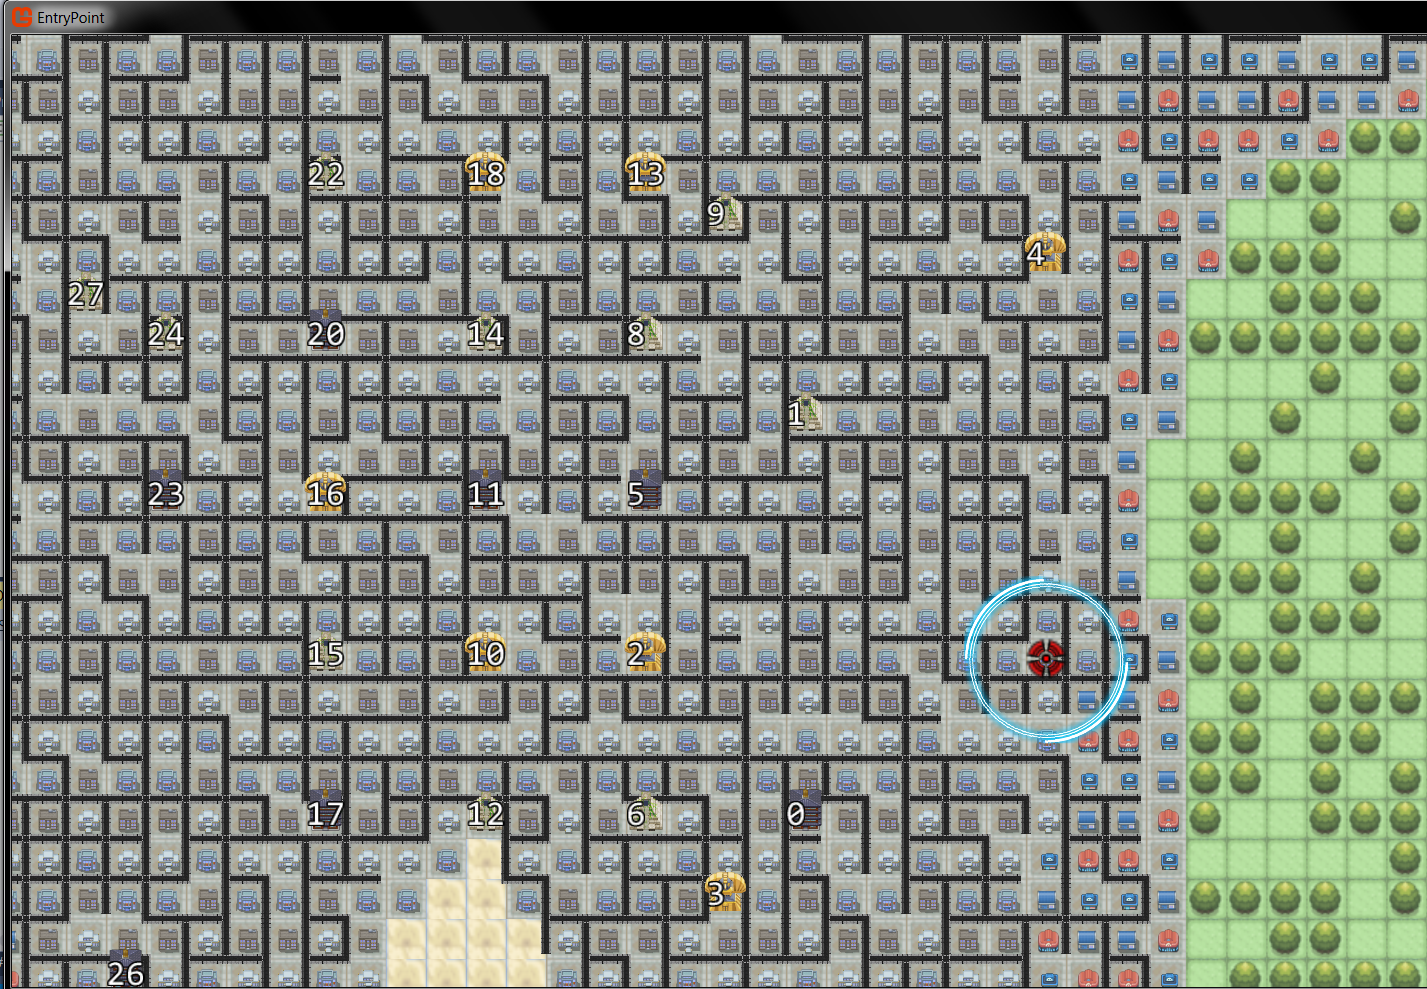
\includegraphics[scale=0.25]{img/exercise1}
\caption{Exercise 1 result}
\label{img:Ex1}
\end{figure}

\newpage
\subsection*{Exercise 2 - Trees}
\textbf{Suggested deadline}: End week 6. \\
\textbf{Points}: 3.

\subsubsection*{Goal}
Find all the special buildings within a specified distance from each house. Create a \textbf{k-d tree} to organize the special buildings positions in advance (like explained in class). Then look up the tree for each of the requested houses (with the associated distance).

\subsubsection*{Function signature} 
\begin{lstlisting}
private static IEnumerable<IEnumerable<Vector2>> FindSpecialBuildingsWithinDistanceFromHouse(IEnumerable<Vector2> specialBuildings, IEnumerable<Tuple<Vector2, float>> houseAndDistances)
\end{lstlisting}

\noindent
This function takes as input a list of special building positions (\texttt{IEnumerable<Vector2> specialBuildings}), a list of pairs made of a house position and the maximum distance for a special building to be selected (\texttt{IEnumerable<Tuple<Vector2, float>> houseAndDistances}), and returns a list of lists of positions (\\ \texttt{IEnumerable<IEnumerable<Vector2>>}) of selected special buildings (one list for each house).\\

\subsubsection*{Result}
As you can see from Figure \ref{img:Ex2}, each selected house is surrounded by a circle that should contain all the special buildings within the distance associated to such house. The buildings you return are highlighted in blue, the houses in red.

\begin{figure}[!h]
\centering
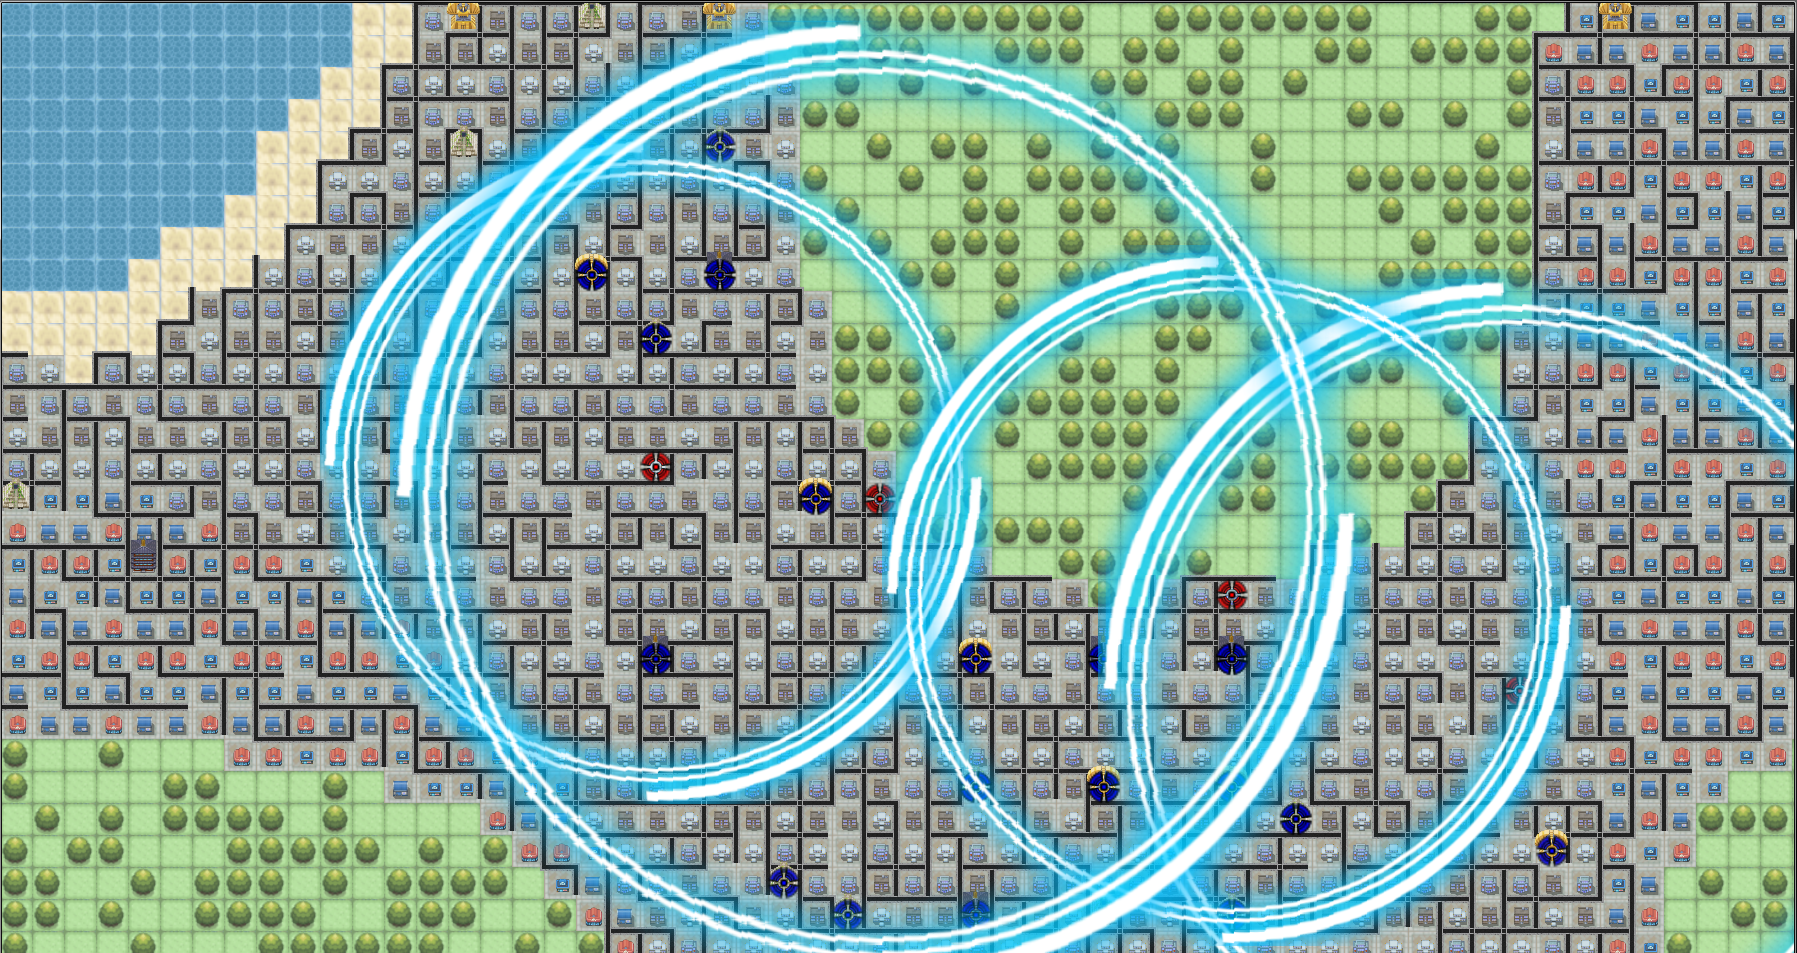
\includegraphics[scale=0.25]{img/exercise2}
\caption{Exercise 2 result}
\label{img:Ex2}
\end{figure}

\newpage
\subsection*{Exercise 3 - Graphs}
\textbf{Suggested deadline}: End week 8. \\
\textbf{Points}: 3.

\subsubsection*{Goal}
Find the shortest path(s) from a specified house to other special building(s). The shortest path is made of the road sections to use in order to drive from the house to the special building.\\
\textbf{Remark}: For this assignment \underline{only}, you can choose between two different implementations (Dijkstra or Floyd Warshall).\\
\textbf{Hint:} In both assignments, you have to build the adjacency matrix using the starting point and endpoint of the road sections. The weight of the edge is the distance between the two points.

\subsection*{Option 1: Dijkstra}
In this assignment we want to compute the minimum path between one house and one special building. 

\subsubsection*{Function signature} 
\begin{lstlisting}
private static IEnumerable<Tuple<Vector2, Vector2>> FindRoute(Vector2 startingBuilding, Vector2 destinationBuilding, IEnumerable<Tuple<Vector2, Vector2>> roads)
\end{lstlisting}

\noindent
This function takes as input the position of the house to start from (\texttt{Vector2 startingBuilding}), the position of the destination (\texttt{Vector2 destinationBuilding}), and a list of road sections, each represented as a pair of starting point and endpoint (\texttt{IEnumerable<Tuple<Vector2, Vector2>> roads}), and returns a list of road sections (\texttt{IEnumerable<Tuple<Vector2, Vector2>>}) forming the shortest path between the house and the destination.\\

\subsubsection*{Result} 
As you can see from Figure \ref{img:Ex3-1}, the house is surrounded by a circle and highlighted in red. The path to the destination is highlighted with coloured dots.

\begin{figure}[!h]
\centering
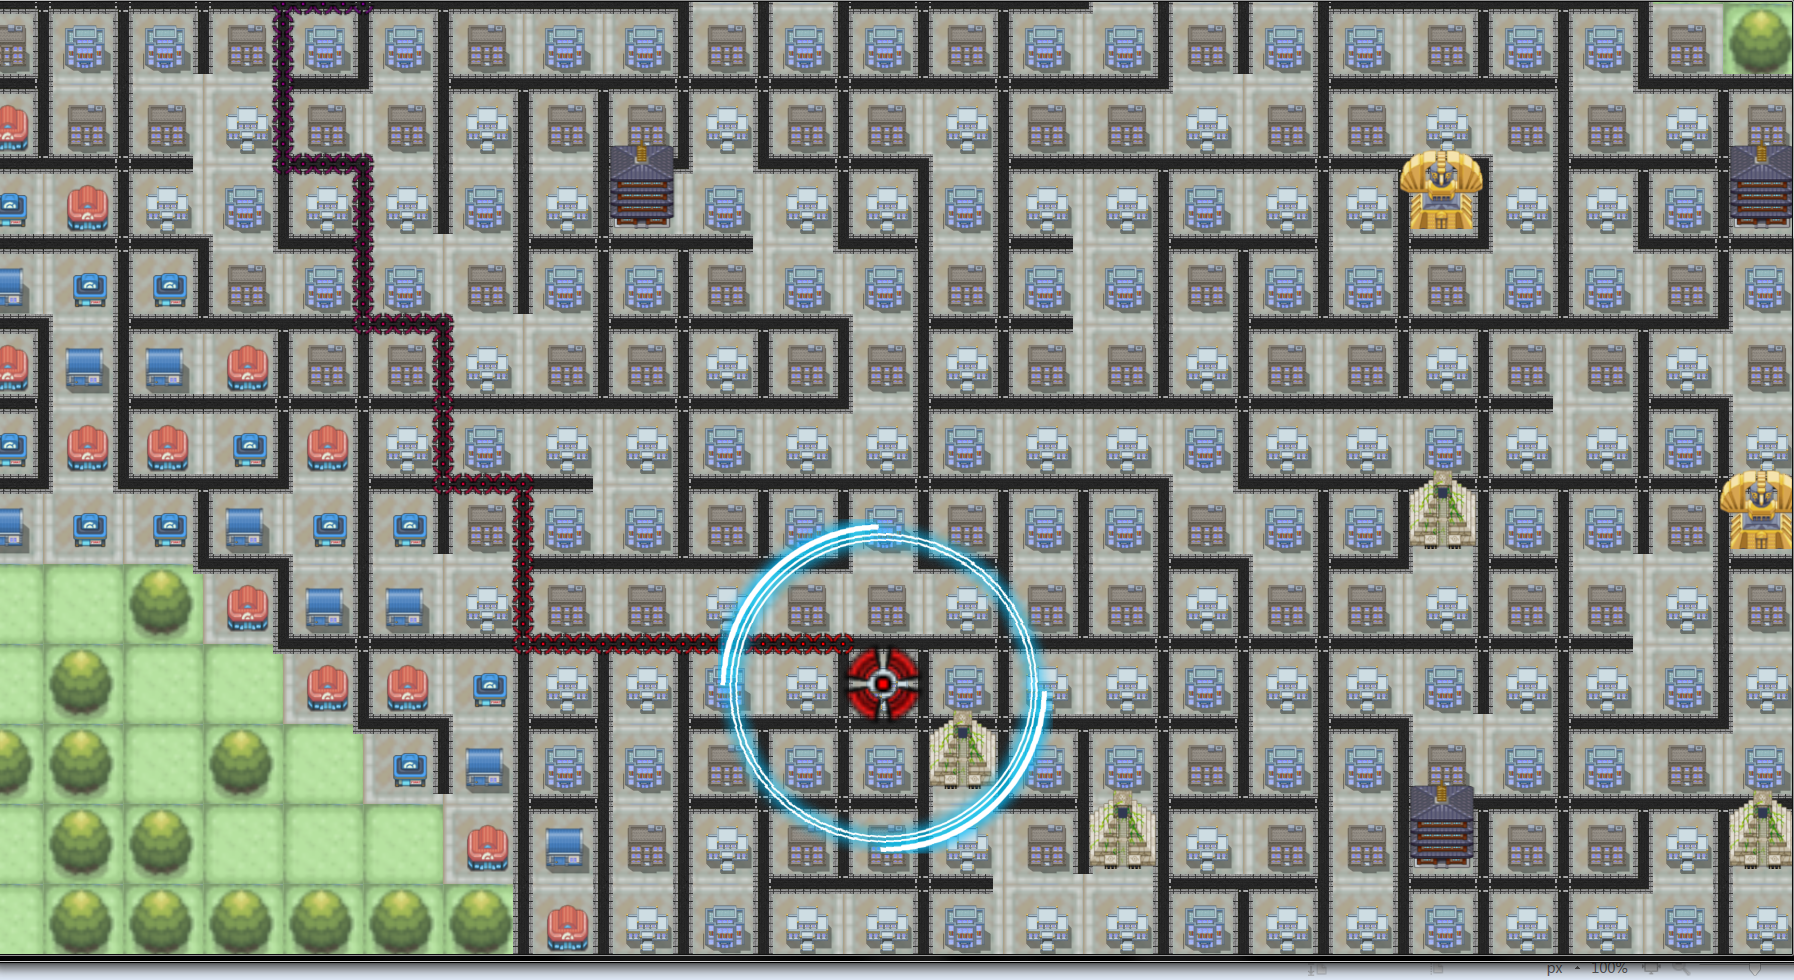
\includegraphics[scale=0.2]{img/exercise3}
\caption{Exercise 3.1 result}
\label{img:Ex3-1}
\end{figure}


\subsection*{Option 2: Floyd Warshall}
In this assignment we want to compute the minimum paths between one house and a list of special buildings. 

\subsection*{Function signature} 
\begin{lstlisting}
private static IEnumerable<IEnumerable<Tuple<Vector2, Vector2>>> FindRoutesToAll(Vector2 startingBuilding, IEnumerable<Vector2> destinationBuildings, IEnumerable<Tuple<Vector2, Vector2>> roads)
\end{lstlisting}

\noindent
This function takes as input the position of the house to start from (\texttt{Vector2 startingBuilding}), the positions of all the destinations (\texttt{IEnumerable<Vector2> destinationBuildings}), and a list of road sections, each represented as a pair of starting point and endpoint (\texttt{IEnumerable<Tuple<Vector2, Vector2>> roads}), and returns a list of shortest paths (\texttt{IEnumerable<IEnumerable<Tuple<Vector2, Vector2>>>}). Each shortest path is referred to one specific destination and is made of a list of road sections.
The function must precompute the all-pairs shortest path with Floyd Warshall algorithm and then extract only the paths requested by the function from the distance and predecessor matrices.\\

\subsection*{Result}
As you can see from Figure \ref{img:Ex3-2}, the house is surrounded by a circle and highlighted in red. The destinations are highlighted in blue. The paths from the house to all destinations are highlighted with coloured dots.

\begin{figure}
\centering
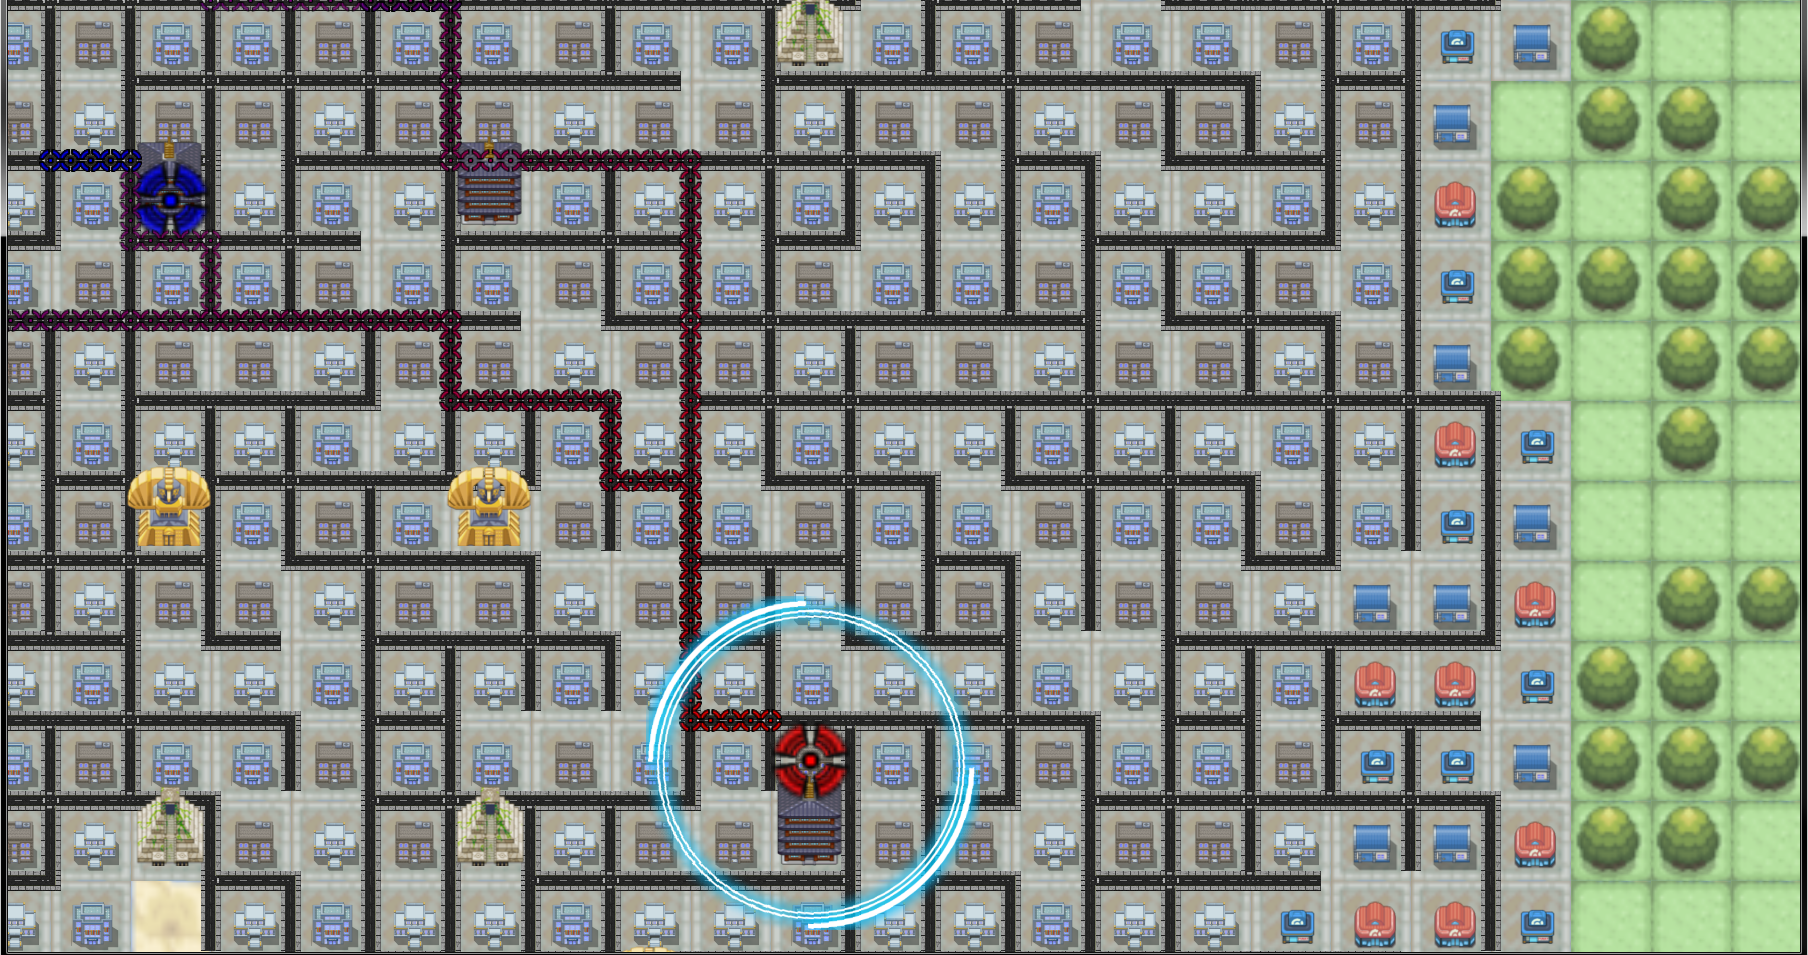
\includegraphics[scale=0.2]{img/exercise4}
\caption{Exercise 3.2 result}
\label{img:Ex3-2}
\end{figure}
\newpage
%\section*{Bijlage 3: Studielast normering in ects}

		Dit hoofdstuk bevat de beschrijving van de procedures om voor beoordeling in aanmerking te komen.\\
		Bijvoorbeeld voldoende aanwezigheid, 80\% van de opdrachten hebben ingeleverd, presentaties hebben verricht etc.\\

		Verder wordt zo gedetailleerd mogelijk beschreven hoe er tot een cijfer wordt gekomen en welke rollen er door docenten en ander betrokkenen hierbij vervuld worden. \\

		Geef een verantwoording van de toets; wat wordt getoetst, waarom is voor deze vorm gekozen.\\

		Vul een toetsmatrijs in voor de toets (zie bijlage).\\

		Beschrijf ook duidelijk de \textbf{herkansingsmogelijkheden}. \\

		Neem in geval van een schriftelijk tentamen een voorbeeldtoets op als bijlage.\\
		Geef daarbij per deelvraag het aantal te verdienen punten aan. \\

		Bij een schriftelijk rapport. Geef de beoordelingscriteria aan met daarbij de mogelijke score en de onderlinge weging. \\

		Toetsduur: \\

		Hoe en wanneer krijgt de student feedback?\\
\printindex


\end{document}
